\documentclass[11pt]{article}
\usepackage{geometry}
\geometry{a4paper, top=27mm, left=25mm, right=20mm, bottom=20mm, headsep=0mm, footskip=12mm}

\usepackage[english]{babel}
\usepackage[utf8]{inputenc}
\usepackage{uniinput}
\usepackage{amsmath,amsfonts,amssymb}
\usepackage{commath}
\usepackage{braket}
\usepackage{mathrsfs}
\usepackage{graphicx}
\usepackage{todonotes}
\title{DMFT with Iterated Perturbation Theory}
\author{Fabian Kugler, Hannes Herrmann and Alessandro Bottero}

\begin{document}
\maketitle

\section{Introduction and Overview}
The aim of this project is to study the metal to Mott-Insulator phase transition exhibited by the Fermi-Hubbard model.

The model consists of a lattice with a single-level \textit{atom} at every site. The electrons can only hop from a site to a nearest neighbour one, and only interact between them if they're at the same site. The Hamiltonian of this model is, therefore, given by:

\begin{equation}
\mathcal{H} = -t\sum_{<i,j>}c_{i,\sigma}^\dagger c_{j,\sigma} + h.c.+ U\sum_i n_{i,\uparrow}n_{i,\downarrow} + \mu\sum_i (n_{i,\uparrow}n_{i,\downarrow})
\end{equation}
where $t$ is the hopping rate, $U$ the strenght of the interaction, varying which we will observe the P.T., and $\mu$ the chemical potential.




This model is studied here by means of Dynamical Mean Field Theory~(DMFT), and the quantity of interest is the local Green's function, given by:

\begin{equation}\label{orGreen's}
G_{ii}^\sigma (\tau - \tau^\prime) = -\braket{Tc_{i\sigma}(\tau)c_{i\sigma}^\dagger(\tau^\prime)} 
\end{equation}
by means of which it will be then possible to compute the \emph{Spectral Function}.

~

The main idea behind the DMFT approach is similar in spirit to the classical mean field approximation and consists in solving the problem of a single atom coupled to a thermal bath and mapping this to our original lattice problem via a self-consistency relation.
Such single atom problem is described by the Hamiltonian of a so called \emph{Anderson Impurity Model} (AIM), given by:

\begin{equation}
\mathcal{H}_{AIM} = \mathcal{H}_{atom} + \mathcal{H}_{bath} + \mathcal{H}_{coupling}
\end{equation}
where we have the following:
\begin{equation}\label{AIMH}
\begin{array}{c}
\mathcal{H}_{atom} = Un_\uparrow^cn_\downarrow^c + (\epsilon_0 - \mu)(n_\uparrow^c+n_\downarrow^c) \\ \\ \mathcal{H}_{bath} = \sum_{l,\sigma}\tilde{\epsilon}_la_{l\sigma}^\dagger a_{l\sigma} \\ \\ \mathcal{H}_{coupling} = \sum_{l,\sigma}V_l(a_{l\sigma}^\dagger c_{\sigma} + c_{\sigma}^\dagger a_{l\sigma})
\end{array}
\end{equation}
here, the the $a_l$'s describe the fermionic degrees of freedom of the bath, while the $\tilde{\epsilon_l}'s$ and the $V_l$'s are parameters which must been chosen appopriately (such that the impurity Green's funtion of \eqref{AIMH} coincides with the local lattice one) and enter through the hybridisation function:

\begin{equation}
\Delta(i\omega_n) = \sum_l\frac{|V_l|^2}{i\omega_n - \tilde{\epsilon}_l}
\end{equation}
how it can be seen from the effective action for the system, obtained integrating out the bath degrees of freedom:
\begin{equation}
S_{eff} = -\int_0^\beta\int_0^\beta d\tau d\tau^\prime\sum_\sigma c_\sigma^\dagger(\tau)\mathscr{G}_0^{-1}(\tau-\tau^\prime)c_\sigma(\tau^\prime) + U\int_0^\beta d\tau n_\uparrow(\tau)n_\downarrow(\tau)
\end{equation}
where we have defined:
\begin{equation}
\mathscr{G}_0^{-1}(i\omega_n) = i\omega_n + \mu - \epsilon_0 - \Delta(i\omega_n) 
\end{equation}

At this point come into play the mean field approximation. First of all, we notice that we can define a local self-energy for the interacting Green's function of the effective AIM, $G(\tau-\tau^\prime)$, via:

\begin{equation}\label{s_imp}
\Sigma_{imp}(i\omega_n) \equiv \mathscr{G}_0^{-1}(i\omega_n) - G^{-1}(i\omega_n)
\end{equation}
And, of course, we can also consider the self-energy of our origina lattice problem, defined from \eqref{orGreen's}, via:
\begin{equation}\label{not_summed_over}
G(\bold{k},i\omega_n) = \frac{1}{i\omega_n + \mu - \epsilon_0 - \epsilon_{\bold{k}} -\Sigma(\bold{k},i\omega_n)}
\end{equation}
with:
\begin{equation}
\epsilon_\bold{k} \equiv t\sum_je^{i\bold{k}\cdot(\bold{R_i}-\bold{R_j})}
\end{equation}
The approximation, now, consists of saying that the lattice self-energy coincides with the impurity self-energy, resulting in vanishing off-diagonal elements of $\Sigma_{latt}$:

\begin{equation}
\Sigma_{ii} \simeq \Sigma_{imp} ~ , \Sigma_{i\neq j} \simeq 0
\end{equation}
which is a consistent approximation only given that it uniquely determines the local Green's function, which, by assumption, is the impurity problem Green's function. We, therefore, sum \eqref{not_summed_over} over $\bold{k}$ to obtain \eqref{orGreen's}, and use \eqref{s_imp} to arrive to the self-consistency relation:
\begin{equation}
\sum_\bold{k}\frac{1}{\Delta(i\omega_n)+G(i\omega_n)^{-1}-\epsilon_\bold{k}} = G(i\omega_n)
\end{equation}

This is the idea behind the DMFT approach. In practice one use an iterative procedure, following the loop: 
\begin{enumerate}
\item start with an initial guess for $\mathscr{G}_0$ (i.e. for $\Delta$);
\item compute the AIM Green's function $G_{imp}$ (by means of perturbation theory, in our case up to second order) $\rightarrow$ $\Sigma_{imp}$ is computed;
\item compute the lattice problem local Green's function $G_{loc}$;
\item update $\mathscr{G}_0$ via $\mathscr{G}_{0,new}^{-1} = G_{loc}^{-1} + \Sigma_{imp}$;
\item iterate till convergence.
\end{enumerate}
which is what we have done in the project. Finally, once the lattice local Green's function has been obtained for the set of values $\{i\omega_n\}$, we fit it using the Padé approximation, and, eventually, we are able to compute the Spectral Function, via analytic continuation of this fit.




\section{The impurity problem in 2\textsuperscript{nd} order perturbation theory}
\label{sec_impsolv}

Translating the Hamiltonian formalism into a functional integral one, we get the action
%
\begin{gather*}
S = \
	%int \sum_{\sigma} \bar{c}_{\sigma} (\tau) \partial_{\tau} c_{\sigma} (\tau) 
	%+ H_{\text{atom}} ( \bar{c}_{\sigma} (\tau), c_{\sigma} (\tau))
	%+ \sum_{l, \sigma} \bar{a}_{\sigma} (\tau) \partial_{\tau} a_{\sigma} (\tau) \\
	%+ H_{\text{\text{bath}}} ( \bar{a}_{\sigma} (\tau), a_{\sigma} (\tau)) 
	%+ H_{\text{\text{coupling}}} (\bar{c}_{\sigma} (\tau), c_{\sigma} (\tau), \bar{a}_{\sigma} (\tau), a_{\sigma} (\tau))
	%\dif \tau
	\int_0^{\beta} \sum_{\sigma} \bar{c}_{\sigma} (\tau) \partial_{\tau} c_{\sigma} (\tau) 
	+ \sum_{l, \sigma} \bar{a}_{\sigma} (\tau) \partial_{\tau} a_{\sigma} (\tau)
	+ \mathcal{H}_{\text{AIM}} \big( \bar{c}_{\sigma} (\tau), c_{\sigma} (\tau), \bar{a}_{\sigma} (\tau), a_{\sigma} (\tau) \big)
	\dif \tau
	\\
	 = \int_0^{\beta}  \mathcal{H}_{\text{atom}} \big( \bar{c}_{\sigma} (\tau), c_{\sigma} (\tau) \big)  \dif \tau 
	+ \sum_{\sigma, \omega} \bar{c}_{\sigma, \omega} 
	\Big( \sum_{l} \frac{V_l}{i\omega - \tilde{\epsilon}_l} - i\omega \Big)
	c_{\sigma, \omega} 
	\\
	+ \sum_{l, \sigma, \omega} \big( \bar{a}_{l, \sigma, \omega} + \frac{V_l}{\tilde{\epsilon}_l - i\omega} \bar{c}_{\sigma, \omega} \big) 
	\big( \tilde{\epsilon_l} - i\omega \big)
	\big( a_{l, \sigma, \omega} + \frac{V_l}{\tilde{\epsilon}_l - i\omega} c_{\sigma, \omega} \big) 
\end{gather*}
%
where some arrangements and usage of the usual Matsubara Fourier transform was made. We use the convention
$
c_{\sigma} (\tau) = \sum_{\omega} e^{-i\omega \tau} c_{\sigma, \omega}
$
where the sum runs over fermionic Matsubara frequencies and a prefactor of $1/ \beta$ is understood, such that $c_{\sigma, \omega}$ has the dimension of inverse energy. Correspondingly, a Kronecker-delta of Matsubara frequencies contains a factor of $\beta$. In the above expression, the bath can easily be integrated out resulting in a bare propagator $G_0$ depending on the parameters $\tilde{\epsilon}_l$, $V_l$ . The case of half filling, $\mu = U/2$, can be equivalently written with a modified interaction and zero chemical potential. Dropping a constant energy term, one has
%
\begin{gather*}
S_{\text{eff}} = S_0 + S_{\text{int}} =
	 - \sum_{\sigma, \omega} \bar{c}_{\sigma, \omega} G_{0, \omega}^{-1}
	c_{\sigma, \omega} 
	%\\
	+ U \sum_{Q} \Big( 
	\underbrace{
	\sum_{k} \bar{c}_{\uparrow,k+Q} c_{\uparrow,k} - \frac{1}{2} \delta_{Q,0} 
	}_{ =: C_Q}
	\Big) \Big(
	\underbrace{
	\sum_{q} \bar{c}_{\downarrow,q-Q} c_{\downarrow,q} - \frac{1}{2} \delta_{Q,0}
	}_{ =: D_{-Q}}
	\Big)
\, .
\end{gather*}

A perturbative expansion of the Green's function exploits (considering w.l.o.g. $c_{\omega} = c_{\uparrow, \omega}$):
%
\begin{equation*}
\beta G(i\omega) = - \langle c_{\omega} \bar{c}_{\omega} \rangle
	= - \frac{\langle c_{\omega} \bar{c}_{\omega} e^{-S_{\text{int}}} \rangle_0}
	{\langle e^{-S_{\text{int}}} \rangle_0}
	= \beta G_{0, \omega} - \frac{1}{2} \langle 
	\big( c_{\omega} \bar{c}_{\omega} + \beta G_{0, \omega} \big)
	 S_{\text{int}}^2 \rangle_0 + \mathcal{O}(U^3)
\, .
\end{equation*}
%
Here, first order terms vanish due to Wick's theorem and the fact that without interaction, the resulting tight-binding model at zero chemical potential is half filled in the ground state,
%
\begin{equation*}
\sum_{\omega} G_{0, \omega} = \langle n_{\sigma} \rangle_0 = \frac{1}{2}
\quad
\Rightarrow
\quad
\langle C_Q \rangle_0 =  \big( \sum_{k} G_{0, \omega} - \frac{1}{2} \big) \delta_{Q,0} = 0
	= \langle D_Q \rangle_0
\, .
\end{equation*}
%
For the contribution to second order, note that only mixed terms survive:
%
\begin{equation*}
\langle D_{-Q_1} D_{-Q_2} \rangle_0
	= \sum_{q_1, q_2}
		\langle c_{\downarrow,q_2} \bar{c}_{\downarrow,q_1-Q_1} \rangle_0
		\langle c_{\downarrow,q_1} \bar{c}_{\downarrow,q_2-Q_2} \rangle_0
	= - \delta_{Q_2, -Q_1} \sum_{q} G_{0,q}G_{0,q+Q_1},
\quad
\end{equation*}
%
\begin{equation*}
\sum_{Q_1} \langle \big( c_{\omega} \bar{c}_{\omega}  +  \beta G_{0, \omega} \big) C_{Q_1} C_{-Q_1} \rangle_0 
	= 2 \sum_{k_1, k_2, Q_1}
		\langle c_{\omega} \bar{c}_{k_1+Q_1} \rangle_0
		\langle c_{k_2} \bar{c}_{\omega} \rangle_0
		\langle c_{k_1} \bar{c}_{k_2-Q_1} \rangle_0
	= -2 \beta G_{0,\omega}^2 \sum_k G_{0,k}
\, .
\end{equation*}

It follows that up to second order, the Green's function is given by
%
\begin{equation*}
G(i\omega) = G_{0, \omega} - U^2 G_{0,\omega}^2 
	\sum_k G_{0,k} \sum_{q} G_{0,q}G_{0,q-k+\omega}
	= G_{0, \omega} + G_{0,\omega}^2 \Sigma_{\omega}\,,
\end{equation*}
%
where we defined the self energy $\Sigma$ in second order perturbation theory. It takes a simpler form in imaginary time space and remembering that we used an effective interaction, we summarize 
%
\begin{equation}
\label{pert_sigma}
\Sigma_\mathrm{eff}(\tau) = - U^2 G_0(\tau)^2 G_0(-\tau)
\quad \quad
\text{with}
\quad 
\mu_{\text{eff}} = 0
\, .
\end{equation}


\section{General computational aspects}

For convenience, we use the Bethe lattice with infinite coordination number in our calculations. With proper rescaling, this leads to the density of states (with band-width $D=2t$)
%
\begin{equation}
D(\varepsilon) = \frac{2}{\pi D} \sqrt{ 1-\frac{\varepsilon^2}{D^2} }\,,
\end{equation}
%
which has the handy property \cite[p. 20]{bethepaper}
\begin{gather}
\int\limits_{-D}^{D} \dif \varepsilon 
\frac{D(\varepsilon)}{DB-\varepsilon} =: \tilde{D}(B) 
\\
\tilde{D}(B) = \frac{2}{\pi D} \left( B \pi + \sqrt{1-B^2}\left[\log{(1-B)}-\log{(B-1)}\right] \right)
\end{gather}
%
Employing \eqref{pert_sigma}, we note the simplified relation for \eqref{Gloc_dos}:
%
\begin{equation}
  G_{\text{loc}} (i\omega_n) = \tilde{D} \Big( \frac{i\omega_n-\Sigma_\mathrm{eff}(i\omega_n)}{D} \Big)
\, .
\end{equation}
For the Bethe lattice \eqref{eq:updateG0} further reduces to \cite[p. 22]{bethepaper}
\begin{equation}
  G_{0,\mathrm{new}}(iω) = i ω - \frac{D^2}{4} G_\mathrm{loc}(iω)
\end{equation}

From the Lehmann representation, one can extract information about the Matsubara Green's function. In terms of eigenstates $\{ | n \rangle \}$ of the full Hamiltonian, one has
%
\begin{equation}
  G(\bold{k},i\omega) = \frac{1}{\mathcal{Z}} \sum_{n,m} \frac{ e^{-\beta E_n} + e^{-\beta E_m} }{i\omega + E_n - E_m} 
	| \langle n | c_{\bold{k}} | m \rangle |^2
\, ,
\end{equation}
%
which implies $G(-i\omega) = G(i\omega)^*$. Moreover, the matrix element ensures that only energies $E_n, E_m$ with states differing in one electron state have non-zero contribution and therefore
%
\begin{align}
\label{G_largefreq}
G(\bold{k},i\omega) \sim \frac{1}{i\omega} \frac{1}{Z} \sum_{n,m} \big( e^{-\beta E_n} + e^{-\beta E_m} \big)
	| \langle n | c_{\bold{k}} | m \rangle |^2 
        = \frac{1}{i\omega} \langle \{ c_\bold{k}, c_\bold{k}^\dag \} \rangle = \frac{1}{i\omega}
\\ \text{for }
| i\omega | \gg \max{(E_n - E_m)} \text{ s.t. } \langle n | c_{\bold{k}} | m \rangle | \neq 0
\, . \nonumber
\end{align}

The spectral function is obtained by analytic continuation from the Matsubara Green's function and has properties proven in a similar way.
%
\begin{equation}
\mathcal{A}(w) = -\frac{1}{\pi} \Im{G(i\omega \rightarrow \omega + i0^+)},
\quad
\mathcal{A}(w) \geq 0,
\quad
\int_{-\infty}^{\infty} \mathcal{A}(w) \dif \omega = 1
\, . \label{eq:Aprops}
\end{equation}
%




\section{Results}
\begin{figure}[t]
	\centering
	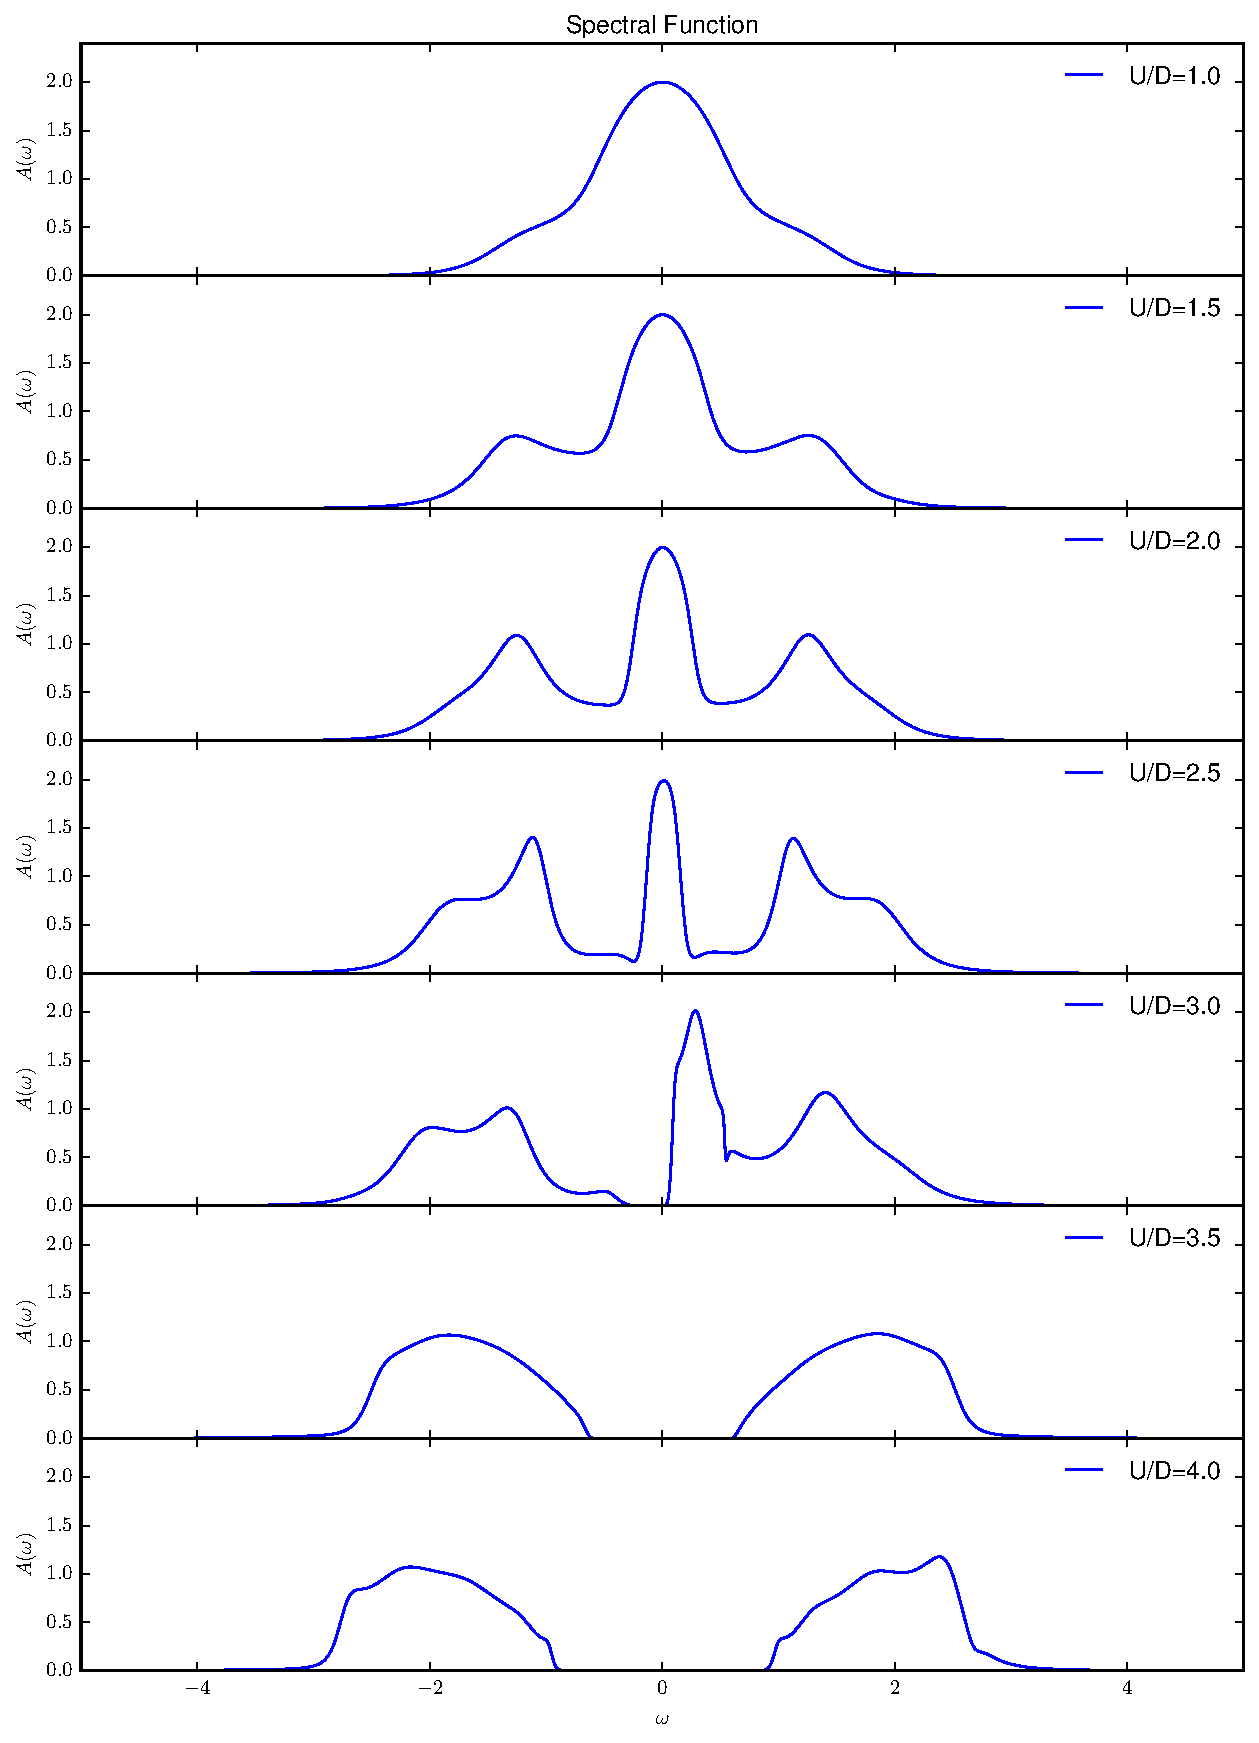
\includegraphics[width=\textwidth]{Mott_transition}
	\caption{Spectral function after analytic continuation. For low interaction parameter $U$ there are single particle excitation??? at zero frequency, therefore the metalic phase. With increasing interaction parameter the spectral function develops a gap at zeros freqency, hence no excitation, ie the insulator phase.}
	\label{fig:spectralf}
\end{figure}
\clearpage






\begin{appendix}
\section{Matsubara Frequencies and Fast Fourier Transform}
In order to solve the impurity model we have to perform several Fourier Transform.
As we consider electrons, the Green's function in imaginary time is antiperiodic by shifts of $\beta$, so we have to use fermionic Matsubara frequencies $ω_n:=\frac{π(2n+1)}{β}$.
The Fourier Transformations are given by (no implicit $\beta$):

\begin{equation}
  G(i ω_n) := \int_0^β dτ G(τ) e^{i ω_n τ} ,
  \quad
  G(τ) = \frac{1}{β} \sum_{i ω_n} G(i ω_n) e^{-i ω_n τ}
\end{equation}
%
For effient calculations we use the FFT-algorithm of the numpy package. Therefore we have to adapt our definitions to the implementation of the numpy library. The numpy library calculates its Fourier Transform by:
\begin{equation}
  A_k = \mathrm{FFT}(a_m) =  \sum_{m=0}^{n-1} a_m \exp\left\{-2\pi i{mk \over n}\right\}
   \qquad k = 0,\ldots,n-1.
\end{equation}
Hence, we discretize the Matsubara Fourier transformation
\begin{align}
  G(i ω_{-n}) &\approx \sum_{k=0}^{N-1} \Delta τ \, G(\Delta τ \, k) \exp{\left(i \frac{π (-2n+1)k}{N}\right)}\\
          &=\frac{\beta}{N} \sum_{k=o}^{N-1} \left( G(\Delta τ \, k)\exp{\left(i π \frac{k}{N}\right)}  \right)  \exp{\left(i \frac{-2 π n k}{N}\right)}\\
	  &= \frac{\beta}{N} \mathrm{FFT}\left( G(\Delta τ \, k)\exp{\left(i π \frac{k}{N}\right)}\right), \label{eq:MFFT}
\end{align}
where $\Delta τ = \frac{\beta}{N}$.
The same can be carried out for the inverse Fourier Tranformations.
\begin{align}
	G(\Delta τ k) &= \frac{N}{β} e^{-i π \frac{k}{N}}\frac{1}{N}\sum_{ω_n}G(i ω_{-n}) e^{i 2π n k/N}\\
	&= \frac{N}{β} e^{-i π \frac{k}{N}}\mathrm{IFFT}(G(iω_{-n})) \label{eq:IMFFT}
\end{align}
\begin{figure}[h]
	\centering
	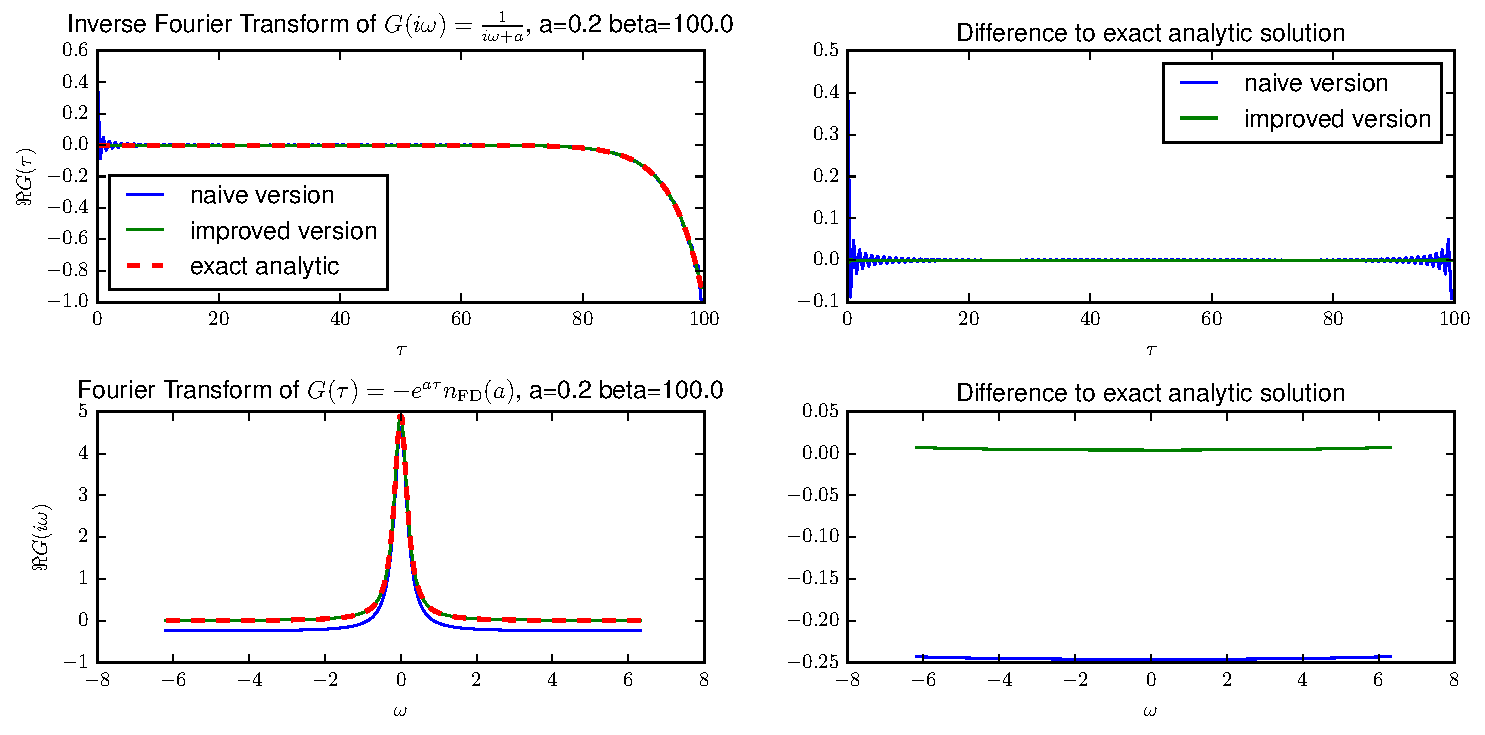
\includegraphics[width=\textwidth]{Matsubara_Fourier_fig}
	\caption{Comparison of the different discretized Fourier Transformations. The improved version, by manually removing the $\frac{1}{i \omega}$ factor, approximates the exact transformation significantly better. }
	\label{fig:fourier_traf}
\end{figure}

Unfortunately the ``naive'' implementations \eqref{eq:MFFT} and \eqref{eq:IMFFT} cause numerical problems, since according to \eqref{G_largefreq} Green's function only decay as $1/ i\omega_n$ in frequency space. As the frequency sum is cut off by the finite number of points used, one strongly increase the accuracy by manually transforming the $1/ i\omega_n$ part. With contour integration, it is commonly shown that ($\tau \neq 0$)
%
\begin{gather}
G(i\omega_n) = \frac{1}{i\omega + a}
\quad \Leftrightarrow \quad
G(\tau) = \Theta(\tau) \frac{- e^{a \tau}}{e^{\beta a}+1} + \Theta(-\tau) \frac{e^{a \tau}}{e^{-\beta a}+1} 
\\
	G(i ω_n) =\frac{1}{i ω_n} \quad ⇔ \quad G(τ)=-\frac{1}{2} + \Theta(-\tau)
	\label{eq:ff_pair}
\, .
\end{gather}
Consequently the improved version of our Fourier transformation is given by subtracting and adding the relevant terms before and after the transformation.
\begin{align}
	G(i ω_{-n})&= \frac{1}{i ω_{-n}}+\frac{\beta}{N} \mathrm{FFT}\left( \left(G(\Delta τ \, k)+\frac{1}{2}\right)\exp{\left(i π \frac{k}{N}\right)}\right)\\
	G(\Delta τ k)&= -\frac{1}{2}+\frac{N}{β} e^{-i π \frac{k}{N}}\mathrm{IFFT}\left(G(iω_{-n})-\frac{1}{i ω_{-n}}\right)
	\label{eq:improved_fft}
\end{align}
The improvement can be seen in \figref{fig:fourier_traf}, where we compare the exact Fourier transformation of $G(i ω)=\frac{1}{iω+a}$ to our discretized versions. The naiv version shows significant deviations to the analytic solution, whereas our improved version approximates the exact one very well.  


\section{Analytic continuation}
\begin{figure}[htb]
  \begin{center}
    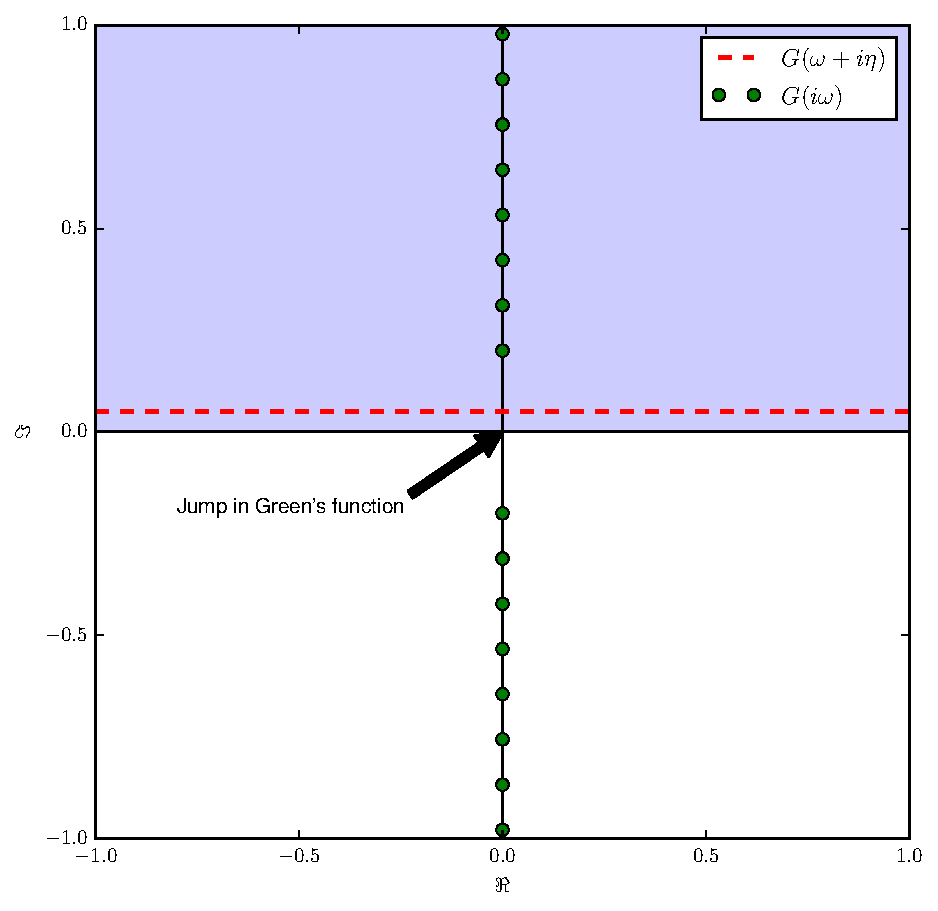
\includegraphics[width=0.7\textwidth]{analytic_continuation}
  \end{center}
  \caption{As the retarded Green's function (red) lies slightly above the real axis and the Matsubara Green's function shows discontinous jumps at zero frequency, we only take the postive frequencies to calculate the Padé approximation. Assuming that the Green's function is analytic in the upper half plane (blue), we expect the anayltic continuation with the rational function to approxmate the retarded Green's function both for positive and negative frequencies. }
  \label{fig:analytic_continuation}
\end{figure}


In order to calculate the spectral function $A$, we have to perform the anlytic continuation of the Matsubara Green's function.
This is a hard problem as we need the functional dependence of $G(iω_n)$ and the only information available is given by discrete points on the imaginary axis.
The central idea is now to interpolate our discrete points by a rational function, called Pade approximation, and use this function to do the analytic continuation. 
An efficient algortihm to calculalte the Padé approximation can be found in \cite{padepaper}. However, as the Padé approximation is continous, whereas the Green's function exhibits non-continous jumps, we have to think about, which values to use for the fit.

In the results of the DMFT-loop we observed discontinous jumps in the Matsubara Green's function at zero frequency.
As we exspect the Greens function to behave non-analytically only on the real axis, we can restrict ourselves on the positive or on the negative frequencies to calculate the fit and use the symmetry of the Greensfunction $G(iω)=G(-iω)^*$ to calculate its values on the opposite half plane.

Since the retared Green's function given by $G(i ω \to w + i o^+)$ lies slightly above the real axis, we can use the positive freqencies on the imaginary axis to calculate the fit and perform the analytic continuation both for positive and negative frequencies of the retarded Green's function as can be seen in \figref{fig:analytic_continuation}.

Furthermore, we homogeneously reduced the number of values to calculate the fit. In some cases this proved to be more stable, which is no surprise, as interpolation polynomials of high degree often shows rapid oscillations.


\end{appendix}

\begin{thebibliography}{9}


\bibitem{bethepaper}
  Antoine Georges, Gabriel Kotliar, Werner Kraut and Marcelo J. Rozenberg
  \emph{Dynamical mean-field theory of strongly correlated fermion systems and the limit of infinite dimensions},
  Revwies of Modern Physics,
  Vol. 68, No. 1,
  1996.
\bibitem{padepaper}
  H.J. Vidberg and J. W. Serene
  \emph{Solving the Eliashberg Equations by Means of N-Point Padé Approximants},
  Journal of Low Temperature Physics,
  Vol. 29, Nos. 3/4,
  1977.
\end{thebibliography}

\end{document}
